\documentclass[00_complete]{subfiles}

%\documentclass[12pt]{report}
\usepackage[utf8]{inputenc}
\usepackage{amsmath,amssymb,amsthm,gensymb,parskip,graphicx,footmisc,csquotes,enumerate,datetime2}
\usepackage[]{libertinus}
\usepackage[breaklinks]{hyperref}
\hypersetup{
  pdfauthor={Moshe Krumbein},
  colorlinks=true,
  linkcolor={black},
  filecolor={black},
  citecolor={black}, %blue
  urlcolor={black}, %blue
}
\usepackage[top=30mm,bottom=30mm,left=30mm,right=30mm]{geometry}
%\setlength{\emergencystretch}{2em} % prevent overfull lines
\providecommand{\tightlist}{%
\setlength{\itemsep}{0pt}\setlength{\parskip}{0pt}}

\renewcommand\qedsymbol{$\blacksquare$}

\theoremstyle{definition}
\newtheorem*{definition}{Definition}
\newtheorem*{theorem}{Theorem}
\newtheorem*{axiom}{Axiom}
\newtheorem*{lemma}{Lemma}

\theoremstyle{remark}
\newtheorem*{note}{Note}
\newtheorem*{symbols}{Symbol}
\newtheorem{example}{Example}[section]
\newtheorem*{claim}{Claim}
\newtheorem*{conclusion}{Conclusion}
\newtheorem*{reminder}{Reminder}

\usepackage{fancyhdr}
\usepackage[italicdiff]{physics}
\MakeOuterQuote{"}

\renewcommand{\chaptermark}[1]{\markboth{#1}{}}

\pagestyle{fancy}

\setlength{\headheight}{14.5pt}
\addtolength{\topmargin}{-2.5pt}

\fancyhf{}
\rhead{Moshe Krumbein}
\lhead{\chaptermark}
\cfoot{\thepage}
\fancyhead[R]{\chaptername~\thechapter}
\fancyhead[L]{\mbox{\leftmark}}

\usepackage[Rejne]{fncychap}
\usepackage{titling}

\makeatletter
\renewcommand{\@chapapp}{\vspace*{-100pt}\huge\thetitle}
\makeatother

\makeatletter
\newcommand{\subtitle}[1]{%
  {\center\vspace*{-60pt}%
  \linespread{1.1}\Large\scshape#1%
  \par\nobreak\vspace*{35pt}}
}
\makeatother

\newcommand{\Chapter}[2]{
    \def\n{#2}
    \setcounter{chapter}{\the\numexpr\n-1}
    \chapter{#1}
    \subtitle{\theauthor~- \thedate}
}

\DeclareMathOperator{\Ima}{Im}
\DeclareMathOperator{\Id}{Id}
\DeclareMathOperator{\cis}{cis}

\newcommand{\Mod}[1]{\ (\mathrm{mod}\ #1)}
\newcommand{\st}[0]{\;\mathrm{s.t.}\;}


\title{Mathematical Methods}
\author{Moshe Krumbein}
\date{Fall 2021}

\begin{document}
\Chapter{Multivariable Functions \texorpdfstring{$\mathbb{R}^{\lowercase{m}}
\to \mathbb{R}$}{Rm to R}}{10}

\section{Introduction}
We are mostly working with $f: \mathbb{R}^2 \to \mathbb{R}$:
$$f(x,y) = z$$
\begin{example}
    \begin{gather*}
     f: z=x^2+y^2 \\
     g: z=\sqrt{1-x^2-y^2} \\
     h: z=\sqrt{x^2+y^2} \\
    \end{gather*}
    \begin{figure}[ht]
    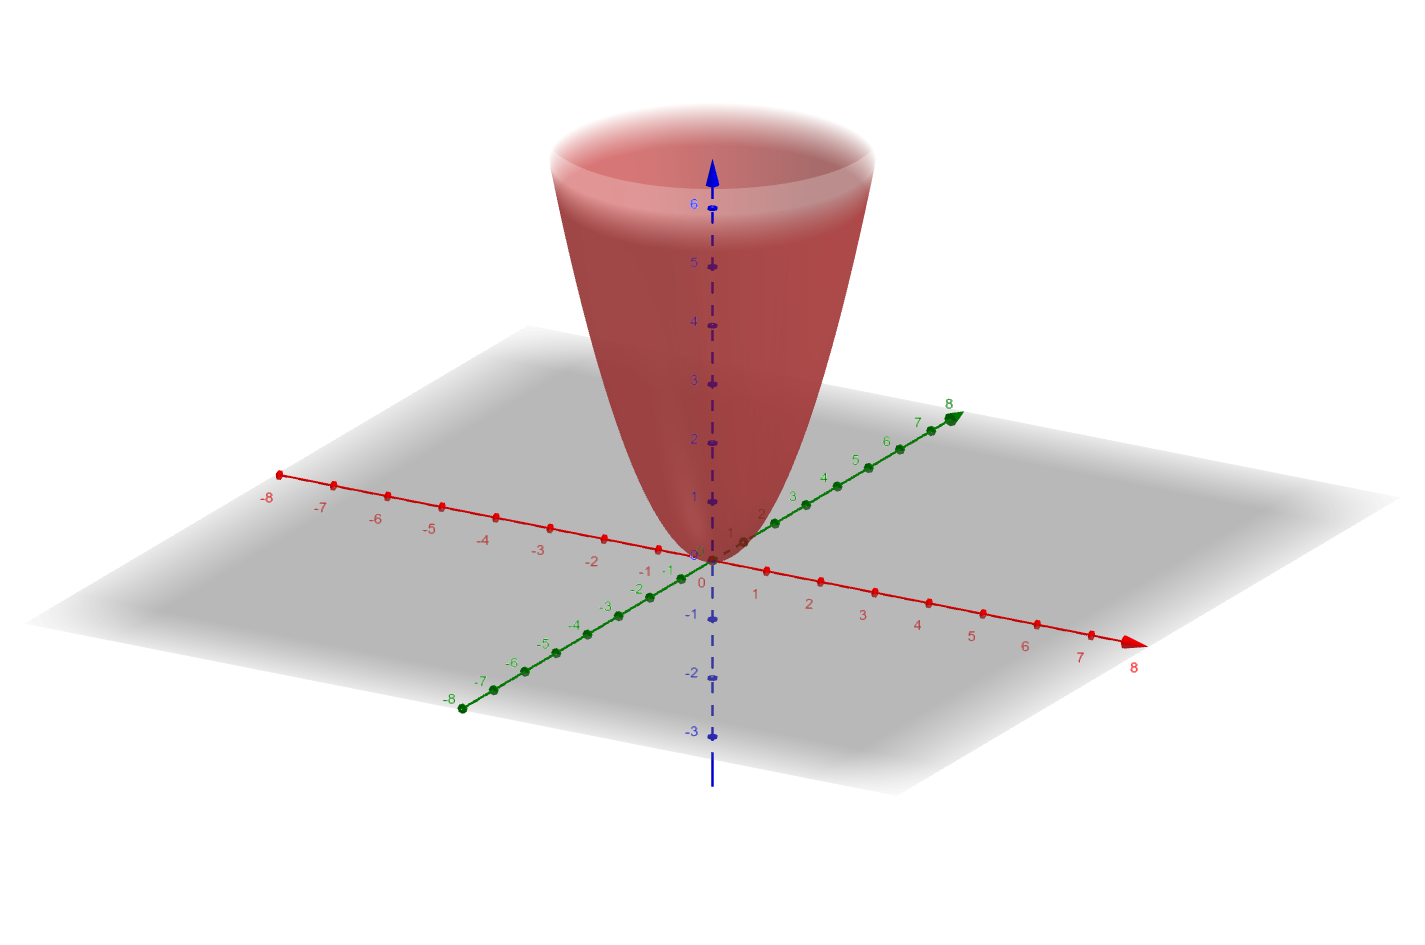
\includegraphics[width=0.33\textwidth]{w10_f}
    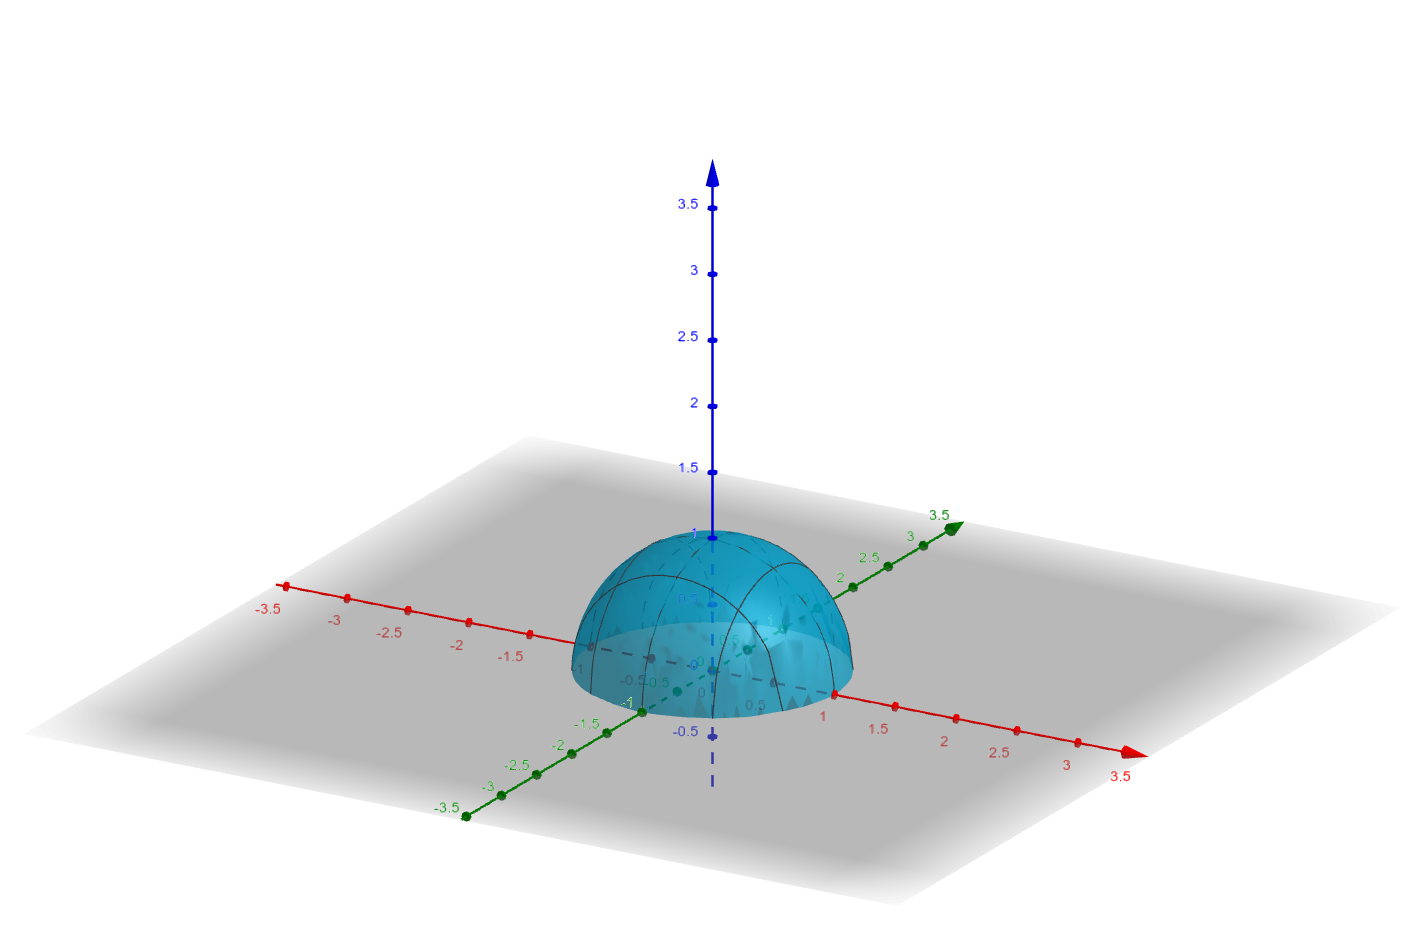
\includegraphics[width=0.33\textwidth]{w10_g}
    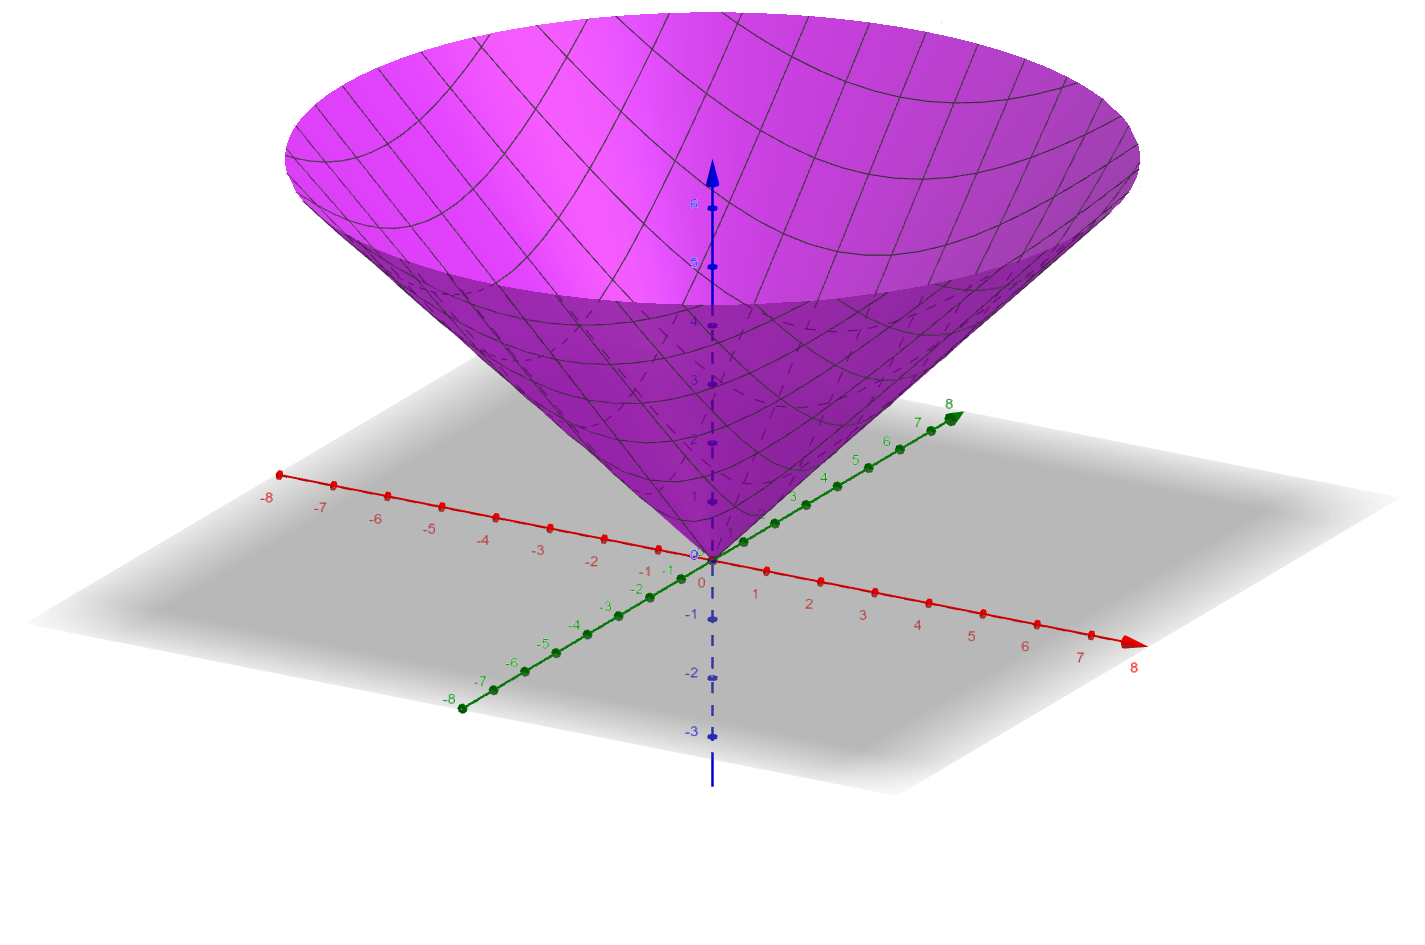
\includegraphics[width=0.33\textwidth]{w10_h}
    \caption{Graphs of the functions $f,g,h$ respectively}
    \end{figure}
    \label{cone}
\end{example}
\section{Domain of Multivariable Functions}
The \emph{domain} is part of the plane $\mathbb{R}^2$.
\begin{example}
    \begin{align*}
        z=x^2+y^2 &\quad \text{Domain: } \mathbb{R}^2 \\
        z=\sqrt{1-x^2-y^2} &\quad \text{Domain: } x^2+y^2\leq 1 \\
        z=\sqrt{x^2+y^2} &\quad \text{Domain: } \mathbb{R}^2 \\
        z=\sin^{-1}(x+y) &\quad \text{Domain: } |x+y| \leq 1 \\
        z=e^x+2y &\quad \text{Domain: } \mathbb{R}^2 \\
        z=\ln(\sin(x^2+y^2)) &\quad \text{Domain: } 2\pi k < x^2+y^2 <(2k+1)\pi
    \end{align*}
\end{example}
\section{Continuity of Multivariable Functions}
\begin{definition}[Continuity of Multivariable Functions]
    $f$ is continuous at the point $(x_0,y_0)$ if for all $(x,y)$ that is ``in
    the neighborhood'' of $(x_0,y_0)$ exists $f(x,y)$ that is ``in the
    neighborhood'' of $f(x_0,y_0)$.
    \begin{example}
        $$f(x,y)=\begin{cases}
            \frac{\sin(x^2+y^2)}{x^2+y^2} &(x,y) \neq (0,0) \\
            1 & (x,y)=(0,0)
        \end{cases}$$
        Is continuous on $\mathbb{R}^2$.
    \end{example}
\end{definition}
\section{Cross Sections of Multivariable Functions with Planes}
Regarding planes of the form $x=x_0$ or $y=y_0$, we simply replace
the variable with the constant in the equation.
\begin{example}
    \begin{gather*}
        z=\sqrt{1-x^2-y^2} \quad x_0=\frac{1}{2} \\
        z = \sqrt{\frac{3}{4}-y^2}
    \end{gather*}
\end{example}
If $z=z_0$:
\begin{example}
    \begin{gather*}
        z=x^2+y^2 \quad z_0=4 \\
        x^2+y^2=4
    \end{gather*}
\end{example}
This also is called a function's \emph{contour line} of height $z_0$.
\section{Partial Derivatives}
\begin{definition}[Partial Derivatives]
    The \emph{partial derivative} of a multivariable function is the derivative
    with respect to only one of its variables (with the others held constant).
\end{definition}
\begin{symbols}
The partial derivative of $f$ with respect to $y$:
    $$\pdv{f}{y},f_y,f_2$$
The partial derivative of $f$ with respect to $x$:
    $$\pdv{f}{x},f_x,f_1$$
\end{symbols}
\begin{example}
    $$f(x,y)=x^3y+e^{2y+x}$$
    Find $f_x(x,y)$ and $f_y(x,y)$.
    \begin{gather*}
        f_x(x,y)=3x^2y+e^{2y+x} \\
        f_y(x,y)=x^3+2e^{2y+x}
    \end{gather*}
\end{example}
\begin{example}[Question 1]
If $f$ is continuous at the point $(x_0,y_0)$, does that mean it's always
partially differential at that point?
\begin{conclusion}
No, a counterexample being a cone, which is continuous everywhere but not
differentiable at its bottom point $(0,0)$ (see $h$ in Example \ref{cone}).
\end{conclusion}
\end{example}
\begin{example}[Question 2]
    Does a function $f$ having both a partial derivative with respect to $x$
    and $y$ ($f_x, f_y$) at a given point imply continuity at that same
    point?
    \begin{conclusion}
        No, counterexample:
        $$f(x,y) = \begin{cases}
            1 & x=0 \text{ or } y=0 \\
            0 & \text{otherwise}
        \end{cases}$$
    \end{conclusion}
\end{example}
\section{Directional Derivatives}
\begin{definition}[Directional Derivatives]
    A \emph{directional derivative} is a partial derivative, but instead of
    finding the derivative with respect to either the $x$ or $y$-axes, we can
    find the derivative and any direction.

    In other words, given a point $(x_0,y_0)$ and a direction $\binom{a}{b}$, we want
    to differentiate $f(x,y)$ in in that direction, at the point $(x_0,y_0)$.
\end{definition}
In order to find the direction derivative, we can express our function $f$ in
terms of $t$:
\begin{gather*}
    \binom{x_0}{y_0}+t\binom{a}{b} \\
    \partial f_{\underline v} \equiv \dv{z}{t}\left(0\right)
\end{gather*}
\begin{note}
    The length of the directional vector has to be equal to $1$:
    $$\left\|\binom{a}{b}\right\|=1$$
\end{note}
\begin{example}
    Find the directional derivative of the function $z=x^2+y$ at the point
    $(2,3)$ in the direction $\displaystyle\binom{\frac{\sqrt 3}{2}}{-\frac{1}{2}}$.
    \begin{gather*}
        f\left(2+\frac{\sqrt 2}{2}t,3-\frac{1}{2}t\right)=\left(2+\frac{\sqrt
            3}{2} t\right)^2 + 3- \frac{1}{2}t
    \end{gather*}
\end{example}
\begin{example}
    $$f(x,y) = \begin{cases}
        \sqrt{x^2+y^2}& y>0 \\
        -\sqrt{x^2+y^2}& y<0 \\
        x & y=0
    \end{cases}$$
    \begin{gather*}
        \hat{\underline e}=\binom{a}{b},\quad f(0+ta,0+tb) = t\sqrt{a^2+b^2} \\
        \partial f_{\hat{\underline
        e}}\left(0,0\right) = \sqrt{a^2+b^2} = 1
    \end{gather*}
\end{example}
\begin{example}
    Differentiate $f(x,y)=x^2y$ at the point $(x_0,y_0)$ in the direction
    $\hat{\underline e}=(a,b)$.
    \begin{gather*}
        g(t)=f(x_0+at,y_0+bt) = (x_0+at)^2(y_0+bt) \\
        g'(t) =\dv{g}{t} = 2(x_0+at)a(y_0+bt) + (x_0+at)^2b \\
        g'(0)=2ax_0y_0+bx_0^2 = \partial f_{\hat{\underline e}}(x_0,y_0)
    \end{gather*}
\end{example}
\begin{example}[Question 3]
    For a function $f$, if there exists a directional derivative in all
    directions at a given point, is $f$ continuous at that point?
    \begin{conclusion}
        No, a counterexample being a function that resembles a piece of paper
        torn in half though still connected at a single point in the middle.
    \end{conclusion}
\end{example}
\section{Differentiability}
\begin{definition}[Differentiability]
   We say that $f(x,y)$ differentiable at $(x_0,y_0)$ if exists a linear
   approximation at that point:
   $$f(x_0+\Delta x,y_0+\Delta y) \approx f(x_0,y_0)+A \Delta x + B \Delta y$$
   In other words, $f(x,y)$ is differentiable at point $(x_0,y_0)$ if there
   exists a tangent plane to that point.
\end{definition}
What are $A$ and $B$ in our equation?
$$f(x_0+\Delta x,y_0) \approx f(x_0,y_0) + A\Delta x$$
We know that:
$$\pdv{f}{x}\/(x_0,y_0) = \lim\limits_{\Delta x \to 0} \frac{f(x_0+\Delta
x,y_0)-f(x_0,y_0)}{\Delta x} =A$$
And likewise:
$$\pdv{f}{y}\/(x_0,y_0) = B$$
Therefore the equation to find the linear approximation is:
$$
    f(x_0+\Delta x,y_0 + \Delta y) \approx f(x_0,y_0) + f_x(x_0,y_0)\Delta x +
    f_y(x_0,y_0)\Delta y
$$
Where the equation for the tangent plane is:
$$
    z=z_0+f_x\cdot (x-x_0)+f_y \cdot (y-y_0)
$$
Suppose that $f$ is differential at the point $(x_0,y_0)$. Find $\partial
f_{\hat{\underline{\binom{a}{b}}}}(x_0,y_0)$.

\begin{gather*}
    g(t)=f(x_0+at,y_0+bt) \approx f(x_0,y_0) + A\cdot at + B \cdot bt \\
    g'(0) = \lim\limits_{\Delta t \to 0} \frac{g(0+t)-g(0)}{\Delta t} =
    \lim\limits_{\Delta t \to 0} \frac{\overbrace{f(x_0+a\Delta t,y_0+b\Delta
    t)-f(x_0,y_0)}^{A\cdot a\Delta t + B\cdot b \Delta t}}{\Delta t} \\
    =A\cdot a + B \cdot b =\boxed{f_x\cdot a + f_y \cdot b}
\end{gather*}
\begin{note}
    This only works for differentiable functions!
\end{note}
Succinctly put:
$$\partial f_{\hat{\underline e}}(x_0,y_0) =
\binom{f_x(x_0,y_0)}{f_y(x_0,y_0)}\cdot \binom{a}{b}$$

How do we know if a function is differentiable at a given point?

If there are partial, continuous derivatives in the "neighborhood" of that
point.
\section{Chain Rule}
\begin{reminder}[Single Variable Functions]
    If $y=f(x)$ and there's a function $g(y)$, then:
    $$\dv{g}{x} = \dv{g}{y} \cdot \dv{y}{x}$$
\end{reminder}
For multivariable functions, there are two chain rules:
\begin{enumerate}
    \item If $f(x,y)$ is \emph{differentiable} and there is a curve on the plane
        $\underline r(t)=(x(t),y(t))$:
        $$\dv{f}{t}=\pdv{f}{x}\cdot \dv{x}{t} + \pdv{f}{y}\cdot \dv{y}{t}$$
        Or in other words:
        $$f'(t)=f_x\cdot x'(t)+f_y\cdot y'(t)$$
        \begin{example}
            $$f(x,y)=xy^2+e^x \quad \underline r(t)=(t^2,t^3)$$
            Using the chain rule:
            \begin{gather*}
            f'(t)=(y^2+e^x)\cdot 2t + (2xy) \cdot 3t^2 \\
            =((t^3)^2+e^{t^2})\cdot 2t + (2t^2t^3)\cdot 3t^2
            \end{gather*}
            Directly:
            \begin{gather*}
                f(x,y)=f(t^2,t^3) = t^8+e^{t^2} \\
                \dv{f}{t}=8t^7+2te^{t^2}
            \end{gather*}
        \end{example}
    \item If $f(x,y)$ is \emph{differentiable} and there are two
        \emph{differentiable} functions $x=x(u,v)$ and $y=y(u,v)$, then:
        \begin{gather*}
            \begin{gathered}
            \pdv{f}{u} = \pdv{f}{x}\cdot \pdv{x}{u}+ \pdv{f}{y}\cdot \pdv{y}{u}\\
            \pdv{f}{v} = \pdv{f}{x}\cdot \pdv{x}{v}+ \pdv{f}{y}\cdot \pdv{y}{v}
            \end{gathered} \quad \vline \quad \begin{gathered}
                f_u=f_x\cdot x_u + f_y\cdot y_u\\
                f_v=f_v\cdot x_v + f_y\cdot y_v\\
            \end{gathered}
        \end{gather*}
\end{enumerate}
In other words, the first chain rule can be written as:
$$f'(t)=\binom{f_x}{f_y}\cdot\binom{x'(t)}{y'(t)}$$
And the second chain rule can be written as:
$$(f_u,f_v)=\begin{pmatrix}f_x&f_y\end{pmatrix}
\begin{pmatrix}x_u&x_v\\y_u&y_v\end{pmatrix}$$
A nice use of the chain rule is for \emph{implicit functions}:

Given the function $f(x,y)=0$, and we consider the contour line $0$ (which is the
curve). We consider the following curve:
$$x=x \quad y=y(x)$$
And how we differentiate with respect to $x$ (which is our $t$ in this case):
$$f_x\cdot \dv{x}{x} + f_y\cdot \dv{y}{x}=0 \implies
\boxed{\dv{y}{x}=-\frac{f_x}{f_y}}$$
\begin{example}[Implicit Functions]
    \begin{gather*}
    xe^y+\ln(2x+3y)=0 \\
    \dv{y}{x} = -\frac{e^y+\frac{2}{2x+3y}}{xe^y+\frac{3}{2x+3y}}
    \end{gather*}
\end{example}
\section{Gradient}
\begin{reminder}
    If $f$ is \emph{differentiable} at $(x_0,y_0)$, then the \emph{directional
    derivative} at $(x_0,y_0)$ in the direction $\hat{\underline{\binom{a}{b}}}$
    is:
    $$\partial f_{\hat{\underline{\binom{a}{b}}}}(x_0,y_0)=f_x\cdot a +
    f_y\cdot b = \binom{f_x}{f_y}\cdot\binom{a}{b}$$
\end{reminder}
\begin{definition}[Gradient]
    The vector of partial derivatives of $f$ is called the \emph{gradient} of
    $f$ and is symbolized as $\underline {\grad f}$.
\end{definition}
\begin{example}
    \begin{gather*}
        f(x,y)=x^2y \\
        \underline{\grad f} = \binom{2xy}{x^2}
    \end{gather*}
    And at the point $(1,3)$ the \emph{gradient} is $\binom{6}{1}$.
\end{example}

Assuming $f$ is differential:
\begin{gather*}
    \partial f_{\hat{\underline e}}(x_0,y_0)=\underline{\grad f}(x_0,y_0)\cdot
    \underline{\hat e} = \|\underline{\grad f}\|\cdot \underbrace{\|\hat{\underline
    e}\|}_{1}\cos \alpha = \|\underline {\grad f}\|\cos \alpha
\end{gather*}
Where $\alpha$ is the angle between the $\underline{\grad f}$ and $\hat{\underline
e}$.
\begin{conclusion}
We can draw the following conclusions based on $\alpha$:
    \begin{enumerate}
    \item The maximum directional derivative is when $\hat{\underline
    e}$ is in the same direction as $\underline{\grad f}$
    ($=\|\underline{\grad f}\|$).
    \item The minimum directional derivative is when $\hat{\underline
    e}$ is in the opposite direction as $\underline{\grad f}$
    ($=-\|\underline{\grad f}\|$).
    \item The directional derivative is zero when $\hat{\underline
    e}$ is perpendicular to $\underline{\grad f}$.
    \end{enumerate}
    Additionally, we can also conclude that the gradient is always
    perpendicular to the contour line.
\end{conclusion}
This can help us better understand the graph of $f$ by first drawing out the
contour line and then overlay the field of gradient vectors.
\begin{note}
    If $z=f(x,y)$, then the \emph{normal} of the tangent plane is
    $\begin{pmatrix}
        f_x\\f_y\\-1
    \end{pmatrix}$.
\end{note}
\begin{definition}[Stationary/Critical Point]
    A point $(x_0,y_0)$ where the \emph{gradient} is zero or doesn't exist is
    called a \emph{stationary} or \emph{critical point} of $f$.

    A \emph{critical point} is:
    \begin{enumerate}[a.] \tightlist
        \item A \emph{local minimum}
        \item A \emph{local maximum}
        \item A \emph{saddle point}
    \end{enumerate}
\end{definition}
\begin{example}
    \begin{gather*}
        f(x,y)=x^3+y^3-3x-3y \\
        f_x=3x^2-3=0 \quad f_y = 3y^2-3=0
    \end{gather*}
    There are four \emph{critical points}: $(\pm1,\pm1)$.
    \begin{align*}
        (1,-1) &
    \end{align*}
    For $(1,-1)$, we'll take a close point $(1+h,-1+k)$:
    \begin{gather*}
        f(1+h,-1+k)=(1+h)^3+(-1+k)^3-3(1+h)-3(-1+k)=\boxed{3h^2-3k^2+h^3+k^3}\\
        f(1,-1)=0
    \end{gather*}
    We see that at the point $(1,-1)$ it isn't the minimum or maximum in its
    neighborhood, and therefore it is a \emph{saddle point}.
\end{example}

\section{High Order Partial Derivatives}
\begin{example}
    \begin{gather*}
        f(x,y)=e^{x^2y} \\
        f_x=2xye^{x^2y} \\
        f_y=x^2e^{x^2y}
    \end{gather*}
    \begin{symbols}
    $$
    \begin{gathered}
        \frac{\partial^2f}{\partial x^2}=\pdv{\pdv{f}{x}}{x}=f_{xx} \\
        \frac{\partial^2f}{\partial y\partial x}=\pdv{\pdv{f}{x}}{y}=f_{xy}
    \end{gathered}\quad \vline \quad
    \begin{gathered}
        \frac{\partial^2f}{\partial y^2}=\pdv{\pdv{f}{y}}{y}=f_{yy} \\
        \frac{\partial^2f}{\partial x\partial y}=\pdv{\pdv{f}{y}}{x}=f_{yx}
    \end{gathered}
    $$
    \end{symbols}
    We find of the derivative of each one with respect to $x$ and $y$:
    \begin{align*}
        f_{xx}=2ye^{x^2y}+4x^2y^2e^{x^2y} & \quad
        f_{xy}=2xe^{x^2y}+2x^3ye^{x^2y} \\
        f_{yx}=2xe^{x^2y}+2x^3ye^{x^2y} & \quad
        f_{yy}=x^4e^{x^2y}
    \end{align*}
    We notice here that $f_{xy}=f_{yx}$.
\end{example}
\begin{theorem}
    If $f_{xy}$ and $f_{yx}$ are defined surrounding $(x_0,y_0)$, then they are
    equal.
\end{theorem}
\begin{theorem}[Taylor's Theorem for Multivariate Functions]
    We are trying to find an approximation to $f(x_0+h,y_0+k)$.

    We define $u(t)=f(x_0+th,y_0+tk)$, which is a single variable function,
    which we can find a Taylor polynomial for.
    \begin{reminder}
        Maclaurin polynomial of $u(t)$:
        $$u(0)+u'(0)t+\frac{u''(0)}{2!}t^2+\dots$$
    \end{reminder}
    \begin{gather*}
        u'(t)=f_x\cdot x'(t)+f_y\cdot y'(t)=hf_x+kf_y \\
        u''(t)=\dv{f_x}{t}\cdot h + \dv{f_y}{t}\cdot k = (f_{xx}\cdot h +
        f_{xy}\cdot k)h+(f_{yy}\cdot h + f_{yx}\cdot k)k \\
        =f_{xx}h^2+2f_{xy}hk+f_{yy}k^2
    \end{gather*}
    Therefore, an approximation of order 2 (where $t=1$):
    $$f(x_0+h,y_0+k)\approx
    f(x_0+y_0)+(f_xh+f_yk)+\frac{1}{2}(f_{xx}h^2+2f_{xy}hk+f_{yy}k^2)$$
\end{theorem}

\section{Investigating Stationary (Critical) Points}
Suppose $(x_0,y_0)$ is a \emph{stationary} point. (In other words:
$f_x(x_0,y_0)=f_y(x_0,y_0)=0$).

We consider an arbitrary point surrounding $(x_0,y_0)$: $(x_0+h,y_0+k)$.
According the second order approximation we just derived:
$$f(x_0+h,y_0+k)\approx f(x_0+y_0)+
\underbrace{(f_xh+f_yk)}_{=0}
+\frac{k^2}{2}\underbrace{\left(f_{xx}\left(\frac{h}{k}\right)^2
    +2f_{xy}\left(\frac{h}{k}\right)
    +f_{yy}\right)}_{\text{Let's investigate!}}
$$
That second order term is always positive when:
\begin{enumerate} \tightlist
    \item $f_{xx} > 0$
    \item $(2f_{xy})^2-4f_{xx}f_{yy}<0$
\end{enumerate}
That second order term is always negative when:
\begin{enumerate} \tightlist
    \item $f_{xx} < 0$
    \item $(2f_{xy})^2-4f_{xx}f_{yy}<0$
\end{enumerate}
It is sometimes positive and sometimes negative when:
\begin{enumerate} \tightlist
    \item $(2f_{xy})^2-4f_{xx}f_{yy}>0$
\end{enumerate}
\subsubsection{Summary}
If $f_{xx}f_{yy}-f_{xy}^2>0$, then $(x_0,y_0)$ is a local critical point.

In such a case, if $f_{xx}>0$ it is a \emph{minimum} point and if $f_{xx}<0$
then it is a \emph{maximum} point.

Alternatively, $f_{xx}f_{yy}-f_{xy}^2<0$, then $(x_0,y_0)$ is a \emph{saddle}
point.
\begin{note}
    If $f_{xx}=0$, we don't know.
\end{note}
Another way to look at it:
$$\begin{vmatrix}
    f_{xx}&f_{xy}\\f_{yx}&f_{yy}
\end{vmatrix}\to \begin{cases}
    >0 & \text{\emph{extreme} point} \\
    <0 & \text{\emph{saddle} point}
\end{cases}$$
\begin{example}
\begin{gather*}
    f(x,y)=x^3-x-y^2\\
    f_x=3x^2-1=0 \qquad f_y=-2y=0 \\
    x=\pm\frac{1}{\sqrt 3} \quad y=0 \\
    \left(\frac{1}{\sqrt 3},0\right) - \text{saddle point} \quad
    \left(-\frac{1}{\sqrt 3},0\right) - \text{maximum}
\end{gather*}
\end{example}
\section{Critical Points under Constraints}
\begin{theorem}[Weierstrass Extreme Value Theorem]
    If $f(x,y)$ is continuous, on a closed and bounded domain, $f$ has
    \emph{minimum} and \emph{maximum} points.
\end{theorem}
How do we find them? They are either:
\begin{enumerate}[a.] \tightlist
    \item Local \emph{extrema}
    \item They are are on bounds of the domain
\end{enumerate}
\begin{example}
    \begin{gather*}
        f(x,y)=x^4+y^4-2x^2+4xy-2y^2 \\
        D =\{(x,y)\mid -6 \leq x,y \leq 6\} =[-6,6]\times[-6,6]
    \end{gather*}
    First, let's find critical points:
    \begin{gather*}
        f_x=4x^3-4x+4y = 0 \\
        f_y=4y^3-4y+4x = 0 \\
        x=0,\pm\sqrt 2 \quad y=-x \\
        (0,0), (\sqrt 2, -\sqrt 2),(-\sqrt 2, \sqrt 2)
    \end{gather*}
    Now, to investigate the bounds, we can break them up into four parts:
    \begin{gather*}
        x=6, -6 \leq y \leq 6: f'(6,y)=4(y^3-y+6)=4(y+2)(y^2-3y+3) \\
        (6,-2),(6,6),(6,-6)
    \end{gather*}
    And continue to the other sides of the bounds to create one list of all
    potential critical points.

    Finally, we plug in all of the points into our original function and see
    which are the \emph{minimum} and \emph{maximum} points in the bounded region.
\end{example}

\section{Differentials}
\begin{reminder}
    If $z=f(x,y)$ and \emph{differentiable}, then $z\approx z_0+f_x\Delta
    x+f_y\Delta y$, or in other words:
    $$\Delta z \approx f_x \Delta x + f_y \Delta y$$
    Then the \emph{differential} of $z$ is:
    $$\boxed{\dd{z}=f_x\dd{x}+f_y\dd{y}}$$
\end{reminder}
\section{Lagrange Multipliers}
The goal is to find \emph{extrema} of a function $f(x_1,\dots,x_n)$ under
constants $g_1(x_1,\dots,x_n)=g_2(x_1,\dots,x_n)=\dots=g_m(x_1\dots,x_n)$.
\begin{example}
    We want to find the \emph{extrema} of $f(x,y)$ under constraint of
    $g(x,y)=0$.

    Lagrange states the an \emph{extremum} will be at a point under the
    constraint of $g(x,y)=0$ is tangent to the contour line of $f$. In other
    words:
    $$\grad f = \lambda \cdot \grad g$$
    Where $\lambda$ is the \emph{Lagrange multiplier}.
\end{example}
\begin{example}
    Find the \emph{extremum} of $f(x,y,z)=xyz$ on the domain:
    $$D=\{(x,y,z) \mid
    \begin{subarray}{m}
        x+y+z=c \\ z,y,z \geq 0
    \end{subarray}\}$$
    First, $D$ is a closed and bounded region, which means it contains minimum
    and maximum points.

    Our constraints:
    $$\underbrace{x+y+z-c}_{g(x,y,z)}=0$$
    We will now find points such that $\grad f= \lambda \cdot \grad g$. In
    other words:
    \begin{gather*}
    \begin{cases}
        f_x=\lambda g_x \\
        f_y=\lambda g_y \\
        f_z=\lambda g_z \\
        g=0
    \end{cases} \quad \vline \quad
    \begin{gathered}
        yz=\lambda \cdot 1 \\
        xz=\lambda \cdot 1 \\
        xy=\lambda \cdot 1 \\
        x+y+z -c=0
    \end{gathered} \\
    (c,0,0), (0,c,0), (0,0,c), \left(\frac{c}{3},\frac{c}{3},\frac{c}{3}\right)
    \end{gather*}
    For the first three points (the boundary of $f$) we see that $f=0$ (which
    is our minimum) and for our fourth point we see that
    $f(\frac{c}{3},\frac{c}{3},\frac{c}{3})=\frac{c^3}{27}$, which is our maximum.
\end{example}
In a case such that we have more than one constraint ($h=g=0$), we use:
$$\grad f = \lambda \grad g + \mu \grad h$$
\begin{example}
    Find the minimum of $f(x,y,z)=x^2+2y^2+3z^2$ under constraint of $x+y+z=1$.

    Our constraint is closed but not bounded, and therefore we cannot be sure
    if there will be a maximum or minimum within our constraint. Indeed in our
    case, there is no maximum.

    Here we will consider the region $-100 \leq x,y,z \leq 100$. It is clear
    that the minimum will be within this region.

    From here we can find our \emph{extrema} using \emph{Lagrange multipliers}
    and we will see that the one \emph{extremum} we find is indeed the global
    minimum.
\end{example}
\end{document}
